% !TEX root = main_min_disc_dist.tex
\subsection{Pursuit-Evasion Game}

We now consider the pursuit-evasion game described in \cite{Mitchell2005}. In the game player I (the control) tries to avoid being captured by player II (the disturbance) on a two dimensional plane. Each player is modeled as a simple kinematic point object with planar position and heading, fixed linear velocity and controllable angular velocity. Taking player I to be at the origin the states $(x_1, x_2, x_3)$ are the relative position and heading of player II and the dynamics are

\begin{equation}
\begin{split}
&\dot{x_1}= -v_u+v_d \cos x_3 + ux_2\\ 
&\dot{x_2}= v_d \sin x_3 - ux_1\\ 
&\dot{x_3}= d-u
\end{split}
\end{equation}

The state space is over the domain $[-6,20] \times [-10,10] \times [0,2\pi[$ with $\U=[-u_{max},u_{max}]$ and $\D=[-d_{max}, d_{max}]$.

Player I is considered captured when the relative distance (in position) between both players is less than $R>0$, thus the target set is given by

\begin{equation}
\T= \{x| x_1^{2}+x_2^2 < R^2\}
\end{equation}


We first compute the value functions for the MR and MDR on a $41 \times 41 \times 41$ grid, and setting the model parameters to $v_u=v_d=5$, $u_{max}=d_{max}=1$, and $R=5$. This will be referred to as the nominal model $M_n$. A visualization of the zero sub-level set for both $V(x)$ and $Z(x)$ for $\lambda=0.001$ is shown in Fig.~\ref{fig:air3D}.


% \begin{figure}
% 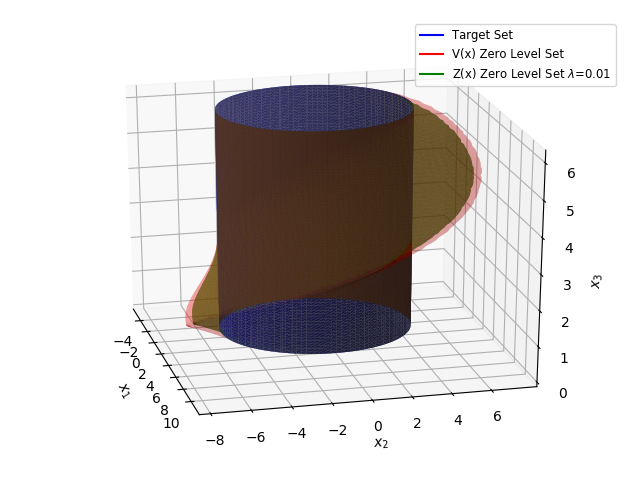
\includegraphics[trim= 2.5cm 0cm 0cm 0.5cm, clip=true,scale=0.65]{air_3D.png}
% \caption{The target set $\mathcal{T}$ is the blue cylinder. The zero sub-level sets of $V$ and $Z$ are in red and green, respectively. The discount rate is $\lambda=0.01$.}
% \label{fig:air3D}
% \end{figure}

\begin{figure*}[h]
    \centering
    \begin{subfigure}[t]{0.3\textwidth}
        \centering
        \includegraphics[trim= 4cm 0cm 0cm 0cm, scale=0.45]{air_3d_v1}
    \end{subfigure}%
    ~ 
    \begin{subfigure}[t]{0.3\textwidth}
        \centering
        \includegraphics[trim= 3cm 0cm 0cm 0cm, clip=true, scale=0.45]{air_3d_v2}
        %\caption{}
    \end{subfigure}
    ~
    \begin{subfigure}[t]{0.3\textwidth}
        \centering
        \includegraphics[trim= 3cm 0cm 0cm 0cm, clip=true, scale=0.45]{air_3d_v3}
        %\caption{}
    \end{subfigure}%
    \caption{The target set $\mathcal{T}$ (blue cylinder), zero sub-level sets of $V$ (red) and $Z$ (green) shown from three different perspectives. The discount rate for $Z$ is $\lambda=0.01$. Note that the zero sub-level set of $Z$ is a subset of the zero sub-level set of $V$.}
    \label{fig:air3D}
\end{figure*}

In the first experiment we compare a multigrid approach to value iteration.  The results are shown in Table~\ref{tab:multigrid_pe}. The experiment and table follows the same structure used for the double integrator model. Similar to the double integrator model, the multigrid approach outperforms value iteration for the pursuit-evasion game.

\begin{table}
\centering
\caption{Pursuit Evasion: Value iteration (VI) with Multigrid} CPU time in seconds
\begin{tabular}{|c| c| c| c| c| }
\hline
\# nodes & Coarse grid & Fine grid &  Fine grid-CS & Multigrid \\ \hline
$40^3$ & $2.068$ & $29.684$ & $24.320$ & $26.388$ \\ \hline
$80^3$ & $33.166$ & $352.099$ & $317.444$ & $350.610$\\ \hline
\end{tabular}
\label{tab:multigrid_pe}
\end{table}

We now construct two other models by tweaking $M_n$: setting $u_{max}=1.5$, which gives the evader an advantage, we get model $M_e$, and setting $d_{max}=1.5$, which gives the pursuer an advantage,  we get model $M_p$. In the final experiment we look at the impact of initializing value iteration with a solution from a similar model. Just like in the previous benchmark example, this experiment is motivated by Section \ref{sec:model_based}, where now $M_e$ and $M_p$ represent two possible models inferred from the system observations. In this context we have just ``learned" that the evader/pursuer is more maneuverable ($M_e$/$M_p$). We compute both value functions with and without setting the initialization to the solution for $M_n$. Again, we refer to this initialization as a warm start. The results are shown in Table~\ref{tab:ws_pe}.

\begin{table}
\centering
\caption{Pursuit Evasion: Value iteration (VI) with Warm Start (WS)} CPU time in seconds
\begin{tabular}{|c| c| c| c| c| c|}
\hline
\# nodes & $M_n$ & $M_e$ &  $M_e$-WS & $M_p$ & $M_p$-WS \\ \hline
$40^3$ & $35.043$ & $32.242$ & $21.483$ & $26.319$ & $23.366$ \\ \hline
$80^3$ & $439.751$ & $416.965$ & $308.821$ & $300.847$ & $296.568$\\ \hline
\end{tabular}
\label{tab:ws_pe}
\end{table}
